\documentclass[a4paper]{report}
\usepackage{url}
\usepackage{graphicx}
%\includeonly{introduction,methodology,relatedwork}
\begin{document}

\title{A Use case for Controlled Languages in Ontology based Knowledge Management}

\author{Pradeep Varma Dantuluri}
\date{August 2010}

\maketitle

\pagenumbering{roman}
\tableofcontents
\listoffigures
\listoftables

\chapter*{Declaration and Disclaimer}
I declare that this thesis is composed by myself, that the work contained herein is my own except where explicitly stated otherwise in the text, and that this work has not been submitted for any other degree or professional qualification except as specified.
The work reported in this thesis is part of research conducted in DERI, Galway within the DERI L\'{i}on-2 project.
Pradeep Varma Dantuluri

\chapter*{Acknowledgements}

\begin{abstract}
Although the Semantic web is steadily gaining in popularity, it remains a mystery to a large percentage of Internet users. This can be attributed to the complexity of the technologies that form its core. Creating intuitive interfaces which completely abstract the technologies underneath, is one way to solve this problem. A contrasting approach is to ease the user into understanding the technologies. We propose a solution which anchors on using controlled languages as interfaces to semantic web applications. This paper describes one such approach for the domain of meeting minutes, status reports and other project specific documents. A controlled language is developed along with an ontology to handle semi-automatic knowledge extraction. The contributions of this paper include an ontology designed for the domain of meeting minutes and status reports, and a controlled language grammar tailored for the above domain to perform the semi-automatic knowledge acquisition and generate RDF triples. This paper also describes two grammar prototypes, which were developed and evaluated prior to the development of the final grammar, as well as the Link grammar, which was the grammar formalism of choice. 
\end{abstract}

\pagenumbering{arabic}

\chapter{Introduction}
%\label{ch:intro}
\section{Motivation}
The Semantic web\footnote{\url{http://www.w3.org/2001/sw/}} aims to simplify the process of building knowledge-based applications by enabling a web of inter-operable and machine-readable data.  This is done by formalizing the descriptions of the structure and semantics of the data available on the web.  The linked data initiative\footnote{\url{http://linkeddata.org/}} is a positive step in that direction, exposing huge amounts of data for further analysis and use by other applications.  However creating and exposing linked data is a task that requires thorough knowledge of various technologies which would be a huge hassle for the novice users.  A solution to this is to create technologies which would enable the average internet user to annotate and embed data in his/her own textual resources.  This work aims to explore the possibility of using controlled natural languages(hereby referred to as CNL) as an interface for semantic annotation, specifically targeting the domain of project documents like meeting minutes,  status reports, etc.  The major goal was to enable novice users to author and annotate text documents simultaneously using a controlled language.  Furthermore, these documents can be parsed to extract the implicit knowledge contained, due to the enforcement of a fixed grammar and vocabulary. This completes the task of converting human-readable controlled language texts to machine-interpretable structured information which could be further exploited. Previously this approach was used to build an annotation tool along with prototypes of the grammar and ontologies for the meeting minutes domain \cite{cnl09}.

\section{Research Goal}
Using CNLs as interfaces to knowledge acquisition applications, soothens the barriers of entry for novice users thereby leading to a greater public involvement.  

The main contributions of the thesis include 
\begin{itemize}

\item{An Annotation Software platform for the knowledge acquisition and management pertaining to the meeting minutes domain}
\item{The development and publishing of an  ontology which models the domain of project documents}
\item{Development of the CLANN grammar using link grammars and the corresponding parser}
\item{A GWT based web interface for the novice users to aid them in authoring texts in Controlled language}
\end{itemize}  

\section{Thesis Layout}



\chapter{Related Work}
%\label{ch:relatedwork}

The proposed work touches upon a combination of topics ranging from CNLs and using them as an interface for Knowledge aquisition, Development and maintainence of ontologies,  the Link grammar formalism, and finally Semantic Web and the Linked data . Essentially the work aims to create a smart application which would allow users to write meeting minutes and status reports in a controlled and restricted version of the english language. This controlled language is machine processable, hence parsed, understood and relevant information is extracted. This information is formatted as RDF data (RDF tripples) using a pre-defined ontology and made accesible through linked data standards.

\section{Semantic Web and Semantic Wikis}



\subsection{Semantic Web}
\subsection{Linked Data web}
\subsection{Wikis and Semantic Wikis}

%%
Other related work involves the application of Controlled Languages
for Ontology/Knowledge base querying, which represent a different task
than that of knowledge creation and editing but are worth mentioning
for completeness sake. Most notably
\emph{AquaLog}\footnote{\url{http://kmi.open.ac.uk/technologies/aqualog/}}
is an ontology-driven,portable question-answering (QA) system designed
to provide a natural language query interface to semantic mark-up
stored in a knowledge base. PowerAqua \cite{LopezMU06} extends
AquaLog, allowing for an open domain question-answering for the
semantic web. The system dynamically locates and combines information
from multiple domains.
%%
Write about Semnatic Web. Write about Linked Data. Explain the reach and progress of Linked data and semantic web with examples. 
The proposed work aims to use Linked data technologies to open up the data of the application and hence connecting to the huge amount of knowledge already availiable on the internet. This enables the users to efficiently exploit the vast amount of information  according to his need.  


\section{Ontologies and Ontology Engineering}
\subsection{Overview of ontologies}
\subsection{Ontology languages}
\subsection{Ontology Engineering}
\subsubsection{Methontology}

Explain ontologies and their need. Explain a few of the methodologies to maintain and develop ontologies. 
The domain of meeting minutes and status reports is modelled as the PDO ontology. Further details are described in the section below.

\section{Controlled Languages and the Semantic Annotation}
\subsection{Controlled Language interfaces for HLT}
%%
''Controlled Natural Languages (CNL)s are subsets of natural language
whose grammars and dictionaries have been restricted in order to
reduce or eliminate both ambiguity and complexity''\cite{schwitter}.
CNLs were later developed specifically for computational treatment and
have subsequently evolved into many variations and flavours such as
Smart's Plain English Program (PEP) \cite{Adr92a}, White's
International Language for Serving and Maintenance (ILSAM)
\cite{Adr92a} and Simplified English\footnote{\url{http://www.simplifiedenglish\-aecma.org/Simplified\_English.htm}}.
They have also found favour in large multi-national corporations,
usually within the context of machine translation and machine-aided
translation of user documentation \cite{schwitter,Adr92a}.
The application of CNLs for ontology authoring and instance
population is an active research area.  \emph{Attempto Controlled
  English}\footnote{\url{http://www.ifi.unizh.ch/attempto/}} (ACE)
\cite{Fuc96a}, is a popular CNL for ontology authoring.  It is a subset
of standard English designed for knowledge representation and
technical specifications, and is constrained to be unambiguously
machine-readable into DRS - Discourse Representation Structure.
, a form of first-order logic.  (It can also be re-targeted to other formal
languages.) \cite{Fuchs06}.  The Attempto Parsing Engine (APE)
consists principally of a definite clause grammar, augmented with 
features and inheritance and written in Prolog \cite{Hoefler04}. 
ACE OWL, a sublanguage of ACE, proposes a means of writing formal,
simultaneously human- and machine-readable summaries of scientific
papers \cite{Kaljurand06,Kuhn06}.
%%

\subsection{Controled Languages for Knowledge Management}
%%
The Rabbit CNL is a another well known CNL\cite{dimitrova08}.  It is similar to 
CLOnE in its implementation but is much more powerful with respect to
ontology authoring capabilities and expressivity. It has also been favorably
evaluated by users in the Ordinance Survey domain but is targeted towards
ontology authoring and not semantic annotations. It has been integrated into
Semantic Media Wiki, the purpose of which to create a user friendly collaborative
ontology authoring using multiple CNLs\cite{Bao09}. 

Other related work (in that creates A-box statements) is WYSIWYM (\textit{What you see is
  what you meant})\cite{Power98}. It involves direct knowledge editing with natural
language directed feedback. A domain expert can edit a knowledge based
reliably by interacting with natural language menu choices and the
subsequently generated feedback, which can then be extended or
re-edited using the menu options. However this differs substantially from semantic annotation.
Similar to WYSIWYM is \emph{GINO} (Guided Input Natural Language Ontology Editor) provides a guided,
controlled NLI (natural language interface) for domain-independent
ontology editing for the Semantic Web. GINO incrementally parses the
input not only to warn the user as soon as possible about errors but
also to offer the user (through the GUI) suggested completions of
words and sentences---similarly to the``code assist'' feature of
Eclipse\footnote{\url{http://www.eclipse.org/}} and other development
environments.  GINO translates the completed sentence into triples
(for altering the ontology) or SPARQL\footnote{\url{http://www.w3.org/TR/rdf-sparql-query/}} queries and
passes them to the Jena Semantic Web framework. Although the guided
interface facilitates input, the sentences are quite verbose and do
not allow for aggregation. Static grammar rules exist for the
controlled language but in addition, dynamic grammar rules are
generated from the Ontology itself as an amendment of additional parsing rules to GINO's grammar in order to guide
the user. This permits the system to handle a domain shift, however
this is heavily dependent on any linguistic data or RDF label data
encoded the ontology \cite{Bernstein06}. 

Finally, \cite{Namgoong07} presents an Ontology based
Controlled Natural Language Editor, similar to GINO, which uses a CFG
(Context-free grammar) with lexical dependencies - CFG-DL to generate
RDF triples.  To our knowledge the system ports only to RDF and does
not cater for other Ontology languages. 
 
%%

\subsection{Semantic Annotation}
Different approaches ( focus on Semi automatic + manual)

%%
While there are a plethora of tools for manual and 
(semi-)automatic tools semantic annotation tools (which apply knowledge based approaches using applied NLP
,machine learning techniques or both to the process), to our knowledge, very little research exists involving the
application of controlled natural language to semantic annotation.
%%

\emph{ " A Controlled Natural Language (CNL) is a subset of a natural language whose grammar and vocabulary has been restricted in order to reduce or eliminate ambiguity and complexity"}\cite{schwitter}. CNLs have been successfully applied as natural language interfaces to enable users to communicate with the application easily without undergoing any rigourous training. 

 CNLs have already been applied to ontology authoring and population \cite{Funk07}.  Previous work by the authors \cite{cnl09} tackle the problem of  applying CNLs to semantic annotation.  The process of semantic annotation according to \cite{sig2003} involves addition or association of semantic data or meta-data to the content, according to an agreed-upon ontology.  Conventionally, work on semantic annotation focused on  two-step approaches where the authoring of a document has to precede the annotation  of the same.  This problem can be overcome by adopting a \emph{latent} annotation\cite{cnl09} approach by the use of controlled languages, which merges both the authoring and annotation steps into one.  The information is encoded in the restricted vocabulary and grammatical structure of the controlled language.  However, preliminary evaluations suggest that annotating every piece of information using a CNL makes the task quite verbose, thereby demotivating the users.  Our previous work explored a simple solution to this by supplementing the CNL using templates which encode implicit domain information.  


\section{Grammar formalisms}
Grammar of a particular language is a list of principles and rules which direct the placement of words to form meaningful sentences of the the language. Grammars of natural langauges have been studied extensively over the past decades, and various formalisms have been defined. They can be broadly categorised into constituent and dependency based formalisms. The fundamental idea of constituency grammars is, words can be grouped into meaningful units or phrases. Context-free grammars (CFG) are the most widely used constituent formalism, described by \cite{Chomsky1956}. CFGs consist of a set of rules representing the grammar of a language, which usually recognize legitimate sentences of the language and generate a tree-like parse structure, breaking the sentence into meaningful phrases.  CFGs are better suited to work with the the syntactic knowledge that can be modelled by grammars, hence forming a backbone of our understanding of the syntax of natural languages. Dependency grammars, however, centre around the relations between various words in a sentence.  The syntactic structure of a sentence is describes in terms of words and various kinds of relations among them, thereby building relations between words instead of genrating a tree-like structure.  Link grammars, described by \cite{sleator1995parsing}, are a special kind of dependency grammars where the links/relations are directional along with an added condition where each word should be linked to atleast one other word.
  
A Link grammar consists of a set of words along with linking requirements of each word. The requirements also encode the directionality for each link. A sentence is said to be part of the grammar if each word in the sentence is linked to atleast one word, while satifying the requirements for each link. Furthermore, the links should not overlap. A more detailed explanation of the Link grammar is given in Sections below.

Our work focusses on extracting meaningful tripples from the input controlled language. This approach places a high importance on the links between various words of a sentence. Hence we preferred a dependency based grammar instead of the usual constituent grammars. 
Why prefer this? elaborate...
Moreover, link grammars are known to work especially well if the lexicon of a grammar is fixed.
who says so? reference..
 Since we aimed to design a controlled language for the domain of meeting minutes and status reports, our lexicon is limited, hence justifying the choice of Link grammars.
 
 Additionally we aim to build a guided input CNL editor which should be able to parse at every step and return a list of possible words that can act as suggestions. An link parsers can be adapted to do so, as they dont need a complete parse for any given sentence. 
 
 %%%%%%%%%%%%%%%%%%%%%%%%%%%%%%%%%%%%%%%%%%%%%5
 




 
% WYSIWYM was used initially in the
% context of the DRAFTER project and the multilingual NLG system
%included in DRAFTER was re-engineered for DRAFTER II \cite{Power98}.
% DRAFTER II and WYSIWYM will most likely be deployed in
%CLEF\footnote{\url{http://www.clinical-escience.org/}} project.  
Perhaps the most closely related technology is the Semantic MediaWiki technology \footnote{More information about Semantic MediaWiki can be found 
at http://semantic-mediawiki.org/wiki/Help:Introduction\_to\_Semantic\_MediaWiki \emph{as accessed on 21/06/09}} have become a popular way of adding semantics to user generated Wiki pages.
 A  traditional wiki creates links between pages without defining the kind of linkage between pages. Semantic MediaWiki allows a user to define the links semantically, thereby adding meaning to links between pages. 
Each concept or an instance has a page in Semantic Wiki, and each outgoing links from this page is annotated with well-defined properties as links. However this kind of approach is not suitable to the kind of 
semantic annotation that we aim for. The Semantic Media Wiki model forces the users to use the wiki pages for content creation and to create a new page for each instance but does not offer a method to annotate arbitrary 
text documents which are not intended to be used as wiki pages. 
Moreover, the relational metadata represented in a Semantic Media Wiki always has the corresponding page as its subject, thereby restricting the creation and description of other relevant entities.





\chapter{Methodology}
%\label{ch:method}


\section{CLANN}
\subsection{Definition}
CLANN (Controlled Language for ANNotation)\footnote{In this document \textit{CLANN} refers to the annotation software platform as well as the grammar} builds on the experiences gained from the previous work, by incorporating redesigned versions of the grammar and the domain ontology.  CLANN is designed to be an end-to-end semantic web application complete with a domain ontology, a persistent layer based on RDF and a user interface for editing and authoring documents.  The domain was expanded to include all the documents in a project specific setting (for example, meeting minutes, status reports, etc).

\subsection{Use case}


\section{PDO Ontology}
%explain the domain of the ontology.
The domain of meeting minutes and status reports was used to engineer an ontology for the purpose of knowledge management.  The initial CLANN prototype was bootstrapped using the the nepomuk ontologies\footnote{\url{www.semanticdesktop.org/ontologies/}} and later extended by the MEMO ontology.  However , the MEMO ontology was only used as a proof of concept implementation of the domain.  Later,  this was completely redesigned and a new ontology PDO (Project Document ontology) was developed in accordance with proper ontology design principles, specifically the Methontology\cite{FLG+97} approach.  The PDO ontology, described using RDFS and OWL-DL, models the inherent structure and concepts of various documents in a project-specific setting, like meeting minutes, status reports etc.   A pictorial representation of the main aspects of the ontology is shown in Figure \ref{figure-pdo}.  \footnote{for a complete specification of the PDO ontology please refer to \url{http://ontologies.smile.deri.ie/pdo} }
% \begin{figure*}
\begin{center}
	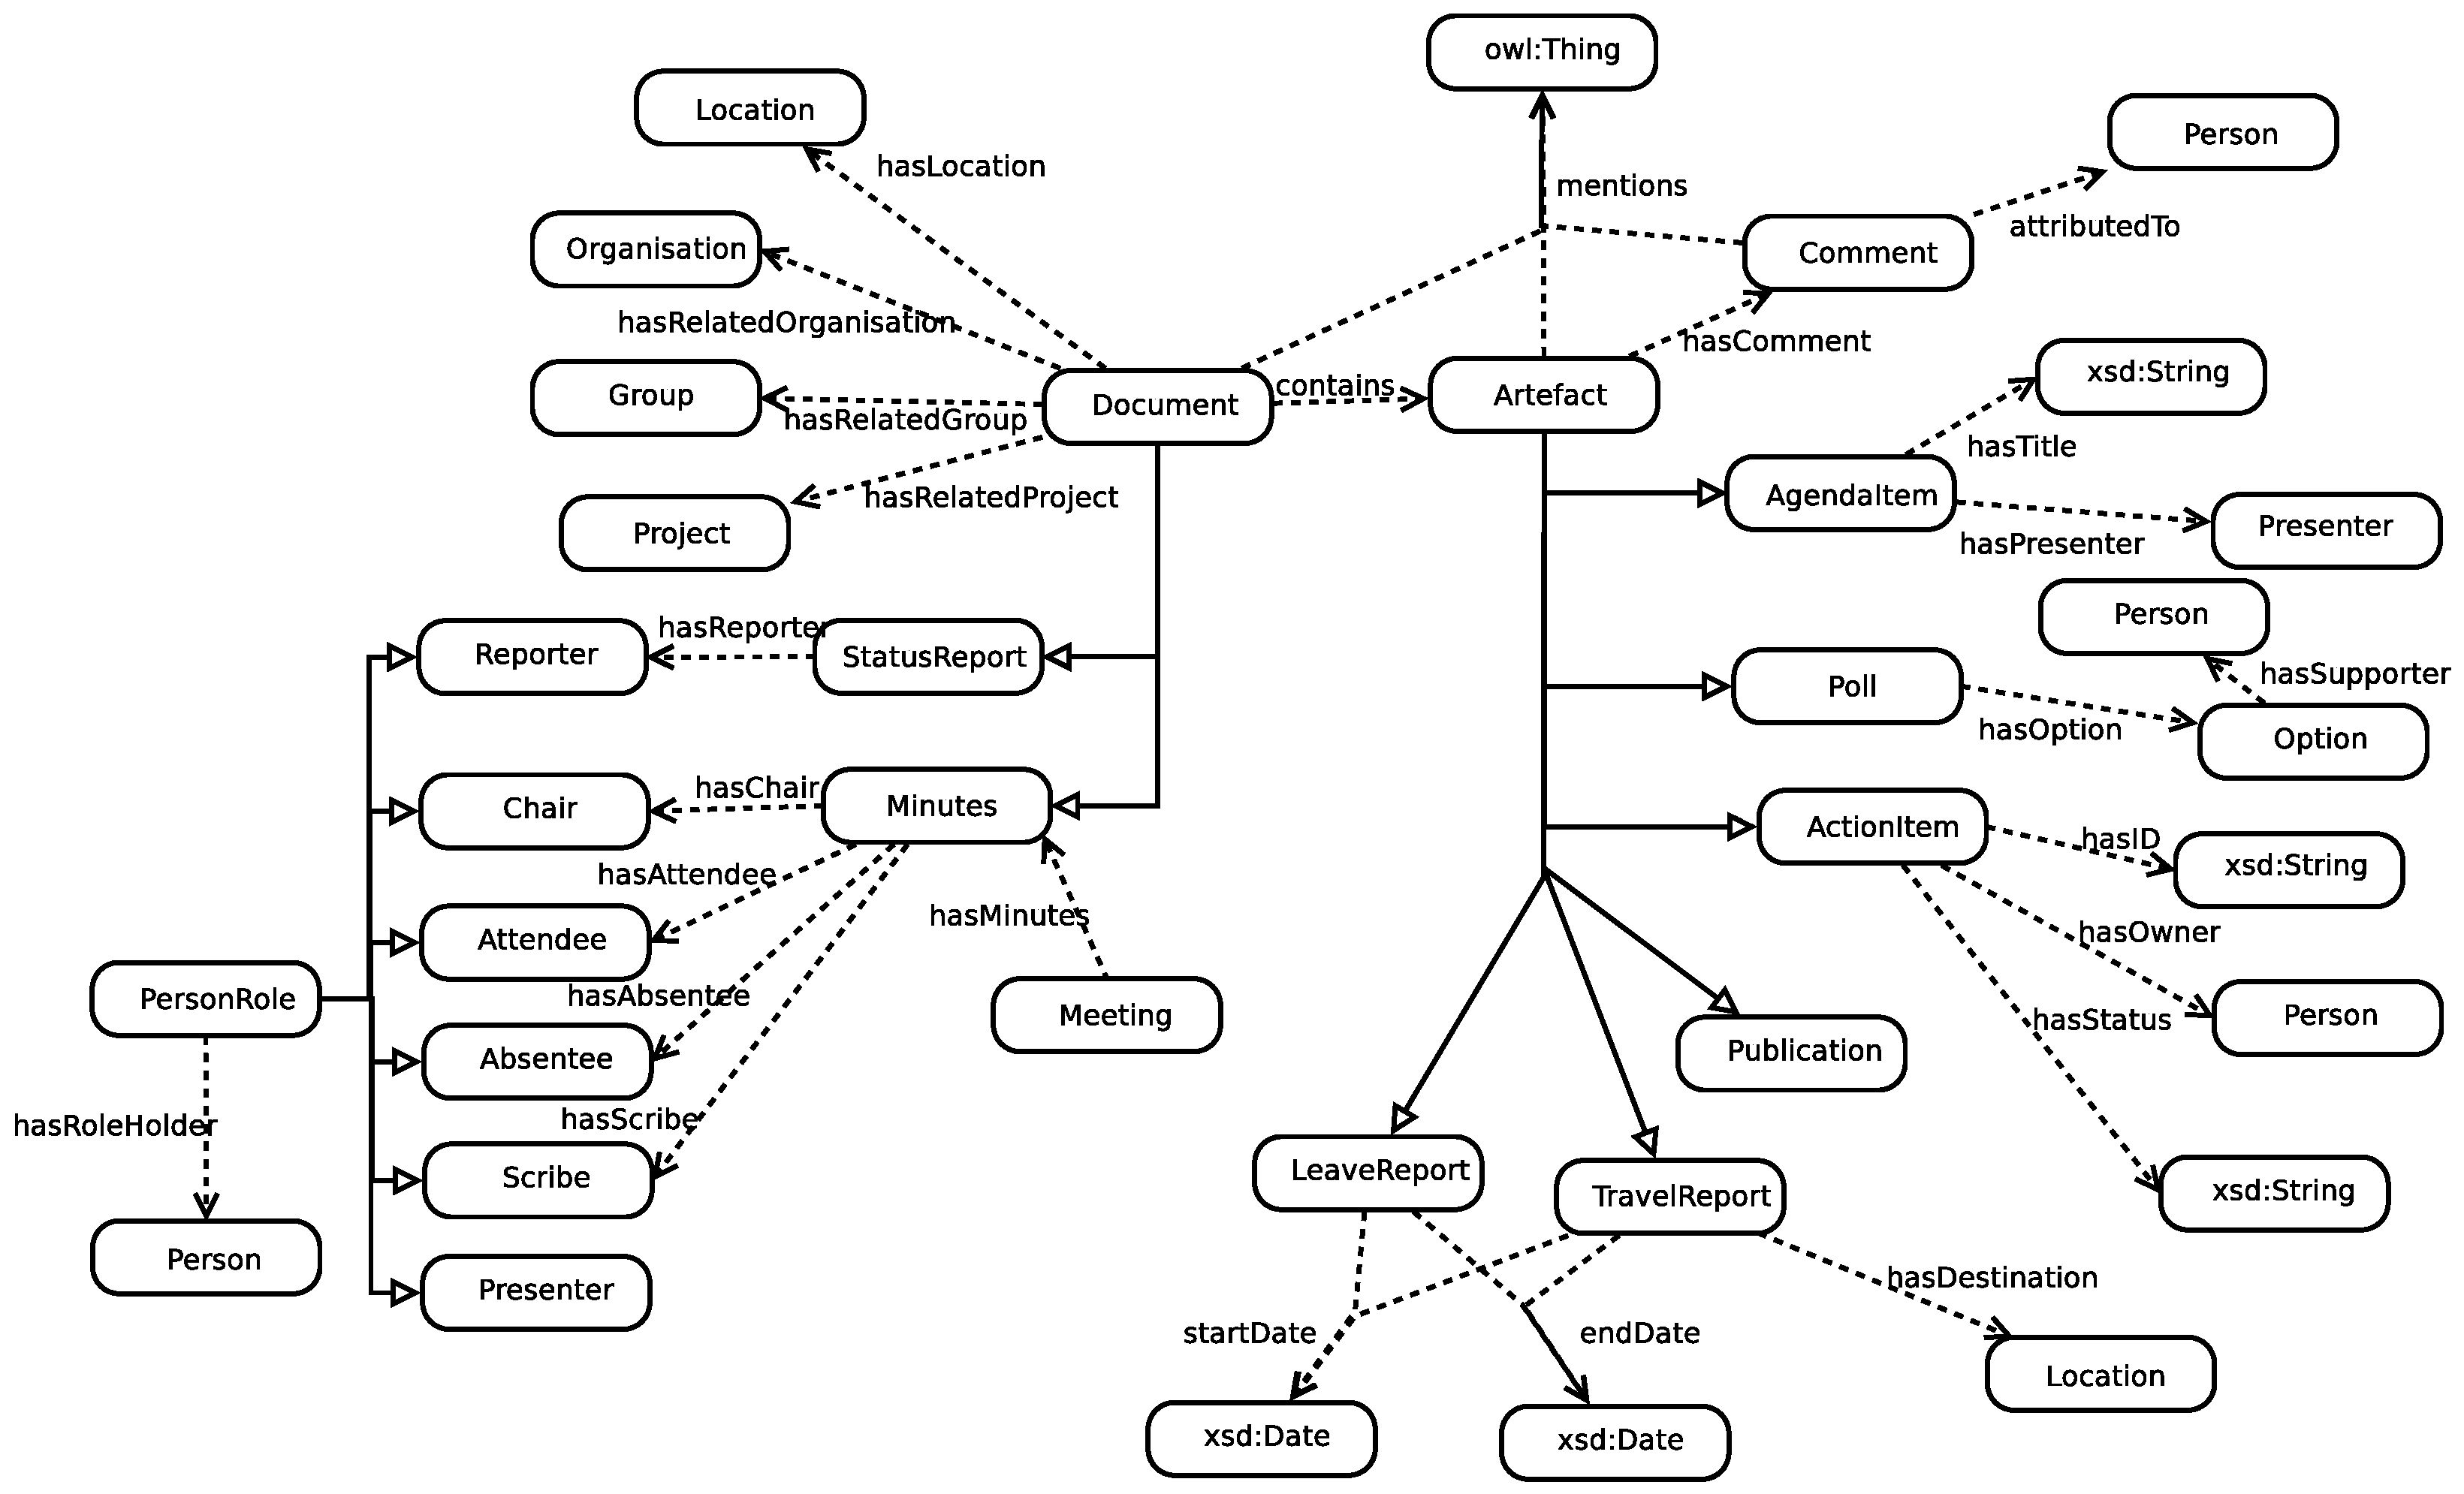
\includegraphics[width=0.8\textwidth]{pdo-v1}
	\caption{Overview of the PDO ontolgoy}
	\label{figure-pdo}
\end{center}
\end{figure*}


\subsection{Design of the ontology}
\subsection{Development and publishing the ontology}


\section{CLANN Grammar}
\subsection{Grammar formalisms}

Various grammar formalisms have been used over the years for understanding natural language.  Phrase structure grammars (PSG), the most widely used formalism, model the inherent structure of the sentences of a language by breaking it into different phrases.  They belong to the class of generative grammars and are composed of a set of productions or rules which break-up the sentences into meaningful phrases.  Dependency grammars(DG), however, concentrate on the links between words without paying attention to the word order.  Structure of a sentence is not broken down into phrases, but determined by adding relations between a head word and its dependent words.  There have been many variations of gramamar formalisms that stemmed out of both PSGs and DGs.  The next few sections describe one such variation of the dependency grammar, the Link grammar, and justifies its selection.

\subsection{Link Grammar}
Link grammars, introduced by \cite{Sleator91}, are a variation of dependency grammars.  Similar to DGs, the link grammars use realtions between words to generate a structure for a sentence.  However, unlike DGs, the links also encode information about directionality and distance.  Moreover, they do not enforce a head-dependent relationship like the DGs.

\cite{Sleator91} defines link grammar as follows:
\begin{quote}\emph{A sequence of words is a sentence of the language if there is a way to draw links between words in such a way that\begin{itemize}
\item the linking requirements of all the words are satisfied,
\item the links do not cross, and
\item the words form a connected graph
\end{itemize} 
}
\end{quote}

The linking requirements of each word are specified as a dictionary, which forms the basis of the link grammar.  Each entry in the dictionary consistes of a word or a group of words belonging to the same grammatical category, appended on the right-hand-side with its linking requirements.  The linking requirements are a series of connectors joined by the logical operators \emph{\&} and \emph{or}.  Each connector denotes the type and direction of the link.  It is a label followed by \emph{+/-} .  \emph{+} denotes a link to the right and \emph{-} denotes a link to the left.  For illustration purposes, an example of a sentence parsed using a very simple link grammar is provided in Figure \ref{figure:link-example}, and an explanation of the same is provided below. 

\begin{figure}[h]
\begin{center}

	\begin{tabular}{l|l}
		\texttt{words} & \texttt{linking requirements}\\
		\hline
		\texttt{the} & \verb#D+#\\
		\texttt{small} & \verb#A+#\\
		\texttt{ate} & \verb#S- & O+#\\
		\texttt{boy apple} & \verb#(A- & D- & S+) or ( D- & O-)#\\
	\end{tabular}
	\begin{verbatim}


 +-----D------+     +----O-----+   
 |     +---A--+--S--+    +--D--+      
 |     |      |     |    |     |              
 the  small  boy   ate  the   apple
\end{verbatim}
	\caption{A sample Link grammar and parse structure.}
	\label{figure:link-example}
\end{center}
\end{figure}



The \emph{D+} connector on the word \emph{the} denotes that \emph{the} is expecting a \emph{D} link to its right.  So It can connect to any word which has a \emph{D-} connector, which, in this case, is either \emph{boy} or \emph{apple}.  The word \emph{ate} has an \emph{\&} operand on \emph{S-} and \emph{O+}.  This means, for the word \emph{ate} to be part of a valid sentence, it should connect to both an \emph{S} connector to its left and an \emph{O} connector to its right.  The case for the nouns \emph{boy} and \emph{apple} is more interesting.  They have two expressions joined by the \emph{or} operand. On closer observation, the first one, \emph{(A- \& D- \& S+)}, models the behavior of a subject noun and the second one, \emph{( D- \& O-)}, models that of an object noun. The reader should also note that the order of the connectors is also valuable. The expression \emph{(A- \& D- \& S+)} also declares the order of linking.  So an \emph{A} link should be made to a word closer than the \emph{D} link. This is illustrated in the parse structure shown in Figure \ref{figure:link-example}. 


\subsection{Why Link Grammar?}

The main design principles for the  CLANN grammar are ease of use and the ability to extend the ontology.  However, the develpoment of the grammar posed different challenges. 

One major priority was to extract RDF tripples from the sentences.  This works very well with the link grammar parse, because the the tripples can directly be extracted by mapping the links.  In the example shown in Figure \ref{figure:link-example}, the tripple \emph{boy ate apple}, can be easily extracted  from the left and right links of the word \emph{ate}.  This is not the case with phrase structure grammars, where extracting dependencies requires detailed ananlysis of the tree structure.   

Another major priority was to develop an intelligent editor on top of the grammar, which supports auto-suggestion and sentence-completion.  An intuitive editor which assists the user while writing the CNL sentences, goes a long way in  helping him to quickly learn the restrictions of the grammar.  This requires an ability to predict text and check the grammatical correctness of partial sentences.  The dictionaries of the link grammar provide valuable information about all the words of the language, which can be exploited for the purpose.
\subsection{Designing the CLANN grammar}
CLANN is designed to enable representing any information that cannot be captured by the templates.  To better explore applicability, two independent prototypes of the grammar CLANN1 and CLANN2 were developed[ref for CNL09]focusing alternatively on usability and expressivity.  This work has eventually led  to CLANN3, which is essentially a merge between the former two grammars, incorporating most of the advantages, albeit a few changes.

\subsubsection{CLANN1 prototype}
CLANN1 is designed with a major focus on usability.  Each sentence adhered to one of the syntactic rules and used a very lenient vocabulary.  This domain vocabulary was derived by corpus analysis using Word Smith tools \footnote{\url{http://www.lexically.net/wordsmith/version5/index.html}} on the document corpus.  This ensured that most of the sentences resembled normal english sentences. CLANN1 is grammatically lax in comparision to typical CNL approaches to knowledge creation. A modified shallow parser is then used to extract the knowledge and instantiate the ontology.
 
\subsubsection{CLANN2 prototype}
CLANN2 was designed with a major focus on expressivity.  It differs from the conventional notion of CNL, whereby the entire document is written in CNL, rather it allows the user to add snippets of CNL text, enclosed in \texttt{"[ ]"}, to the document or associate them to a particular text in the document.These snippets should adhere to a \emph{subject-verb-object} syntax, where the subject is either specified in the snippet or taken from the free text.  The vocabulary for CLANN2 also includes the vocabulary of the ontology, thereby allowing the user to represent any kind of relational meta-data.  This approach was inspired by the CLOnE Language \cite{Funk07}.

The finer details of design and implementation of these grammars are described in \cite{cnl09}.  Both grammars use a common template, described above, which is initially parsed to extract  the inherent meta data of the document (in this case, meeting minutes). 

\subsubsection{CLANN grammar}

 
The CLANN grammar is essentially a combination of CLANN1 and CLANN2, incorporating the snippets of CLANN2 into controlled text of CLANN1 instead of free text.   For other sample documents and information please refer to the project home page\footnote{\url{http://smile.deri.ie/projects/clann}}.


\subsubsection{Templates}
Inorder to supplement the CLANN grammar, we templates which encode implicit domain information, an example of which is shown below.

\begin{minipage}[t]{3.5in}

\texttt{Project Name: <String>\\
Group Name: <String>\\
Date: <Date>\\
Chair: <String>\\
Attendees: (<String>)+\\
Scribe: <String>\\
Action Item:<String>:<String>(:<String>)? (<CNL))+\\
Agenda: <String> (<CNL>)+\\
Poll:<String>:<String> (<String>:<String>)+\\
}
\end{minipage}

These templates were constructed by analysing a collection of in-house meeting minutes and status reports  of the Nepomuk project\footnote{\url{http://dev.nepomuk.semanticdesktop.org/wiki/WikiStart}}.  This approach combines the benefits of the two by using templates for mundane information annotation and CNL for other non-mundane information, consequently minimising the effort and enhancing the user experience.


\section{Design and development of CLANN}
\subsection{CLANN Annotation Platform}
\subsection{Design of the platfrom}
\subsection{Architechture}
\subsection{Modules}
\subsection{Interfaces availiable}
\subsection{Sceenshots}





\subsection{The CLANN grammar}






\chapter{Evaluation}
%\label{ch:evaluation}

\section{Experimental Evaluation}
\subsection{Methodology}
\subsection{Sample quality}
\subsection{Discussion}
\subsection{User feedback}


\chapter{Conclusions and Future Work}
%\label{ch:conc}

\section{Conclusion}
\subsection{Research problem revisited}
\subsection{Further Research}
\subsection{Conclusion}


\bibliographystyle{plain}
\bibliography{mastersthesis}

\end{document}




